\documentclass[crop,tikz]{standalone}
\usetikzlibrary{backgrounds}
\colorlet{blue}{cyan}
\tikzset{
  inverted/.style = {
    color=white,
    background rectangle/.style={fill},
    show background rectangle
  }
}

\usepackage{amsmath}
\tikzset{>=latex}
\usetikzlibrary{calc,patterns,decorations.pathmorphing}

\begin{document}
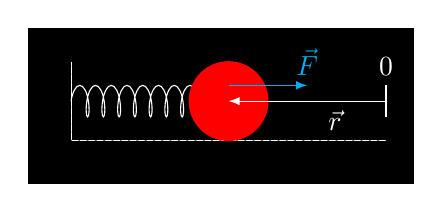
\begin{tikzpicture}[inverted,scale=2]
  % wall
  \draw (-1,0.5) -- (-1,0) -- (1,0);
  \pattern[pattern=north east lines,pattern color=black] (-1.2,0.5)--++(0.2,0)--++(0,-0.5)
    --++(2,0)--++(0,-0.2)--++(-2,0)--++(-0.2,0)--cycle;
  % circle
  \coordinate (c) at (0,0.25);
  \draw[decoration={aspect=0.3, segment length=2mm, amplitude=2mm,coil},decorate] (-1,0.25) -- (c);
  \draw[red,fill] (c) circle (0.25);
  % spring force
  \draw[->,blue] ($(c)+(0,0.1)$) -- ++(0.5,0) node[above]{$\vec{F}$};
  \coordinate (o) at ($(c)+(1,0)$);
  % space vector
  \draw[->] (o) -- node[below, xshift=1em] {$\vec{r}$} (c);
  \draw ($(o)+(0,-0.1)$) -- ++(0,0.2) node[above] {$0$};
\end{tikzpicture}
\end{document}
